\documentclass[10.5pt,a4paper]{article}

\usepackage[margin={1cm,1cm}]{geometry} 
\usepackage{multicol} % For the two column layout
\usepackage{graphicx} % For includegraphics / images command
\usepackage{color}
\usepackage[dvipsnames]{xcolor}
\usepackage{parskip} 
\usepackage[hidelinks]{hyperref} % For clickable hyperlinks (the "hidelinks" part hides the light blue box around hyperlinks)
\usepackage{titlesec} % Needed to set section and subsection header spacing below
\usepackage[T1]{fontenc} % Font encoding
\usepackage[english]{babel} % Load correct hyphenation rules for the English language

\setlength{\columnsep}{1cm} % Central gap between columns
\graphicspath{ {images/} } % Graphics location
\renewcommand*\rmdefault{pag} % Set font
\pagenumbering{gobble} % Disables page numbering

\titlespacing\section{0pt}{12pt plus 4pt minus 2pt}{0pt plus 2pt minus 2pt}
\titlespacing\subsection{0pt}{12pt plus 4pt minus 2pt}{0pt plus 2pt minus 2pt}
\titlespacing\subsubsection{0pt}{12pt plus 4pt minus 2pt}{0pt plus 2pt minus 2pt}


\begin{document}

\begin{center}
	\vspace{1cm}
	\colorbox{Black}{
		\begin{minipage}{18.5cm}
			\begin{center}
			\color{white}
			\vspace{0.3cm}
	             
\includegraphics[width=1\textwidth]{crypto_white.eps}
	        \\[10pt]
			     \textbf{{\LARGE CRYPTOPARTYNEWCASTLE.ORG}}
			\vspace{0.3cm}
			\end{center}
		\end{minipage}
	}
\end{center}

\begin{center}
\vspace{0.5cm}
\textbf{{\LARGE How To Encrypt Your Windows PC}
\vspace{0.5cm}
}\end{center}

\begin{multicols*}{2}

DiskCryptor is a free-and-open-source encryption suite that supports full-disk encryption. Full disk encryption ensures that data on your machines cannot be accessed without your password. This is great for protecting your data if your device is stolen, needs to be submitted for repair, or if you might want to sell or donate it in future.

\begin{center}
	\vspace{0.25cm}
	\colorbox{Maroon}{
		\begin{minipage}{8cm}
			\color{white}
			\vspace{0.1cm}
			\textbf{WARNING:} Please ensure that you make a full backup of your important files \textit{before} following this guide --- in case something goes wrong.
			\vspace{0.1cm}
		\end{minipage}
	}
\end{center}

\section*{Installation}
Head to the following link and locate the installation file for DiskCryptor:

\begin{center}
	\url{https://diskcryptor.net/wiki/Downloads}
\end{center}

Download the installation file and open it to install DiskCryptor.

The default installation settings should be fine, but you can change them if you wish. Restart your machine to finish the installation process.

\section*{Full Disk Encryption}
This section will teach you how to encrypt the whole disk that Windows is installed on.

First, open DiskCryptor from the shortcut that has been installed.

In the \textit{Disk Drives} list, highlight your main drive (this will normally be labelled \textbf{C:}), then press the \textit{Encrypt} button:

\begin{center}
	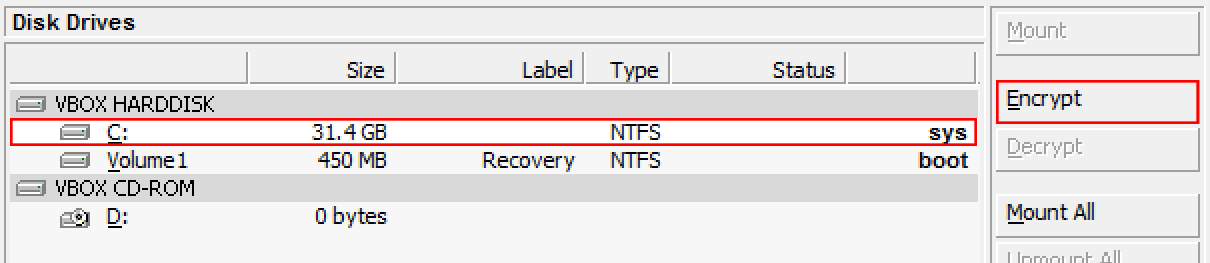
\includegraphics[width=0.40\textwidth]{select-drive.png}
\end{center}

On the next screen, you will be shown some \textit{Encryption Settings}. The default options used are perfectly fine, but you may change them if you have a particular reason to do so:

\begin{center}
	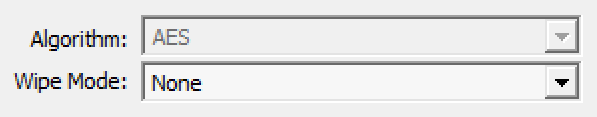
\includegraphics[width=0.40\textwidth]{enc-options.png}
\end{center}

\vspace{1cm} % This is a lazy cheat to push the line below onto the next column so it's not orphaned from the image it refers to
After confirming the above options, you will be shown a window with \textit{Boot Settings}:

\begin{center}
	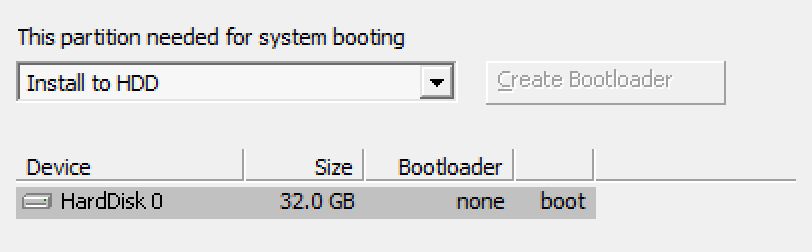
\includegraphics[width=0.40\textwidth]{boot-settings.png}
\end{center}

Again, the default options should be fine for most users, but if you have installed multiple operating systems on your machine please seek additional information online before proceeding with these defaults.

On the final screen before the encryption process starts, you will be asked to choose a password:

\begin{center}
	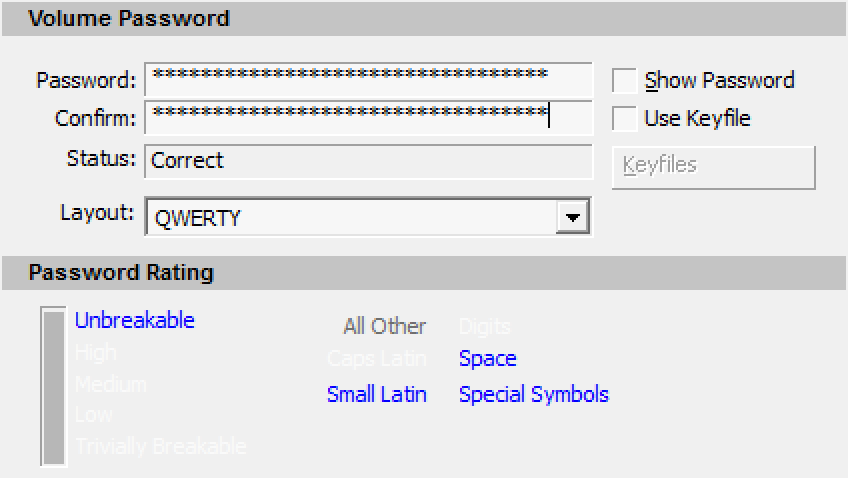
\includegraphics[width=0.40\textwidth]{volume-password.png}
\end{center}

The window offers some helpful hints on the strength of your password as you enter it. When you are satisfied, press 'OK' to begin encrypting.

\begin{center}
	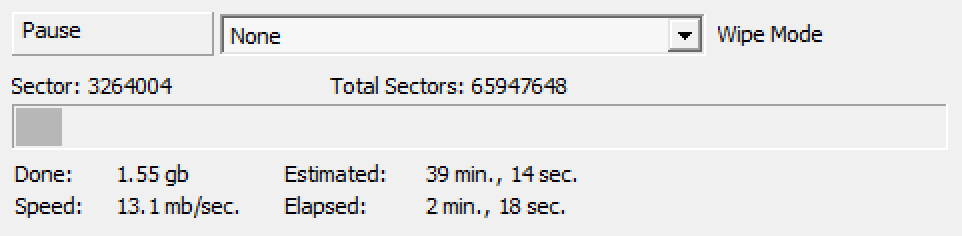
\includegraphics[width=0.40\textwidth]{encrypting.png}
\end{center}

Once the process completes, you will be prompted to restart. During the startup process you should be asked for your password.

You will be asked for this password every time you start your PC. \textbf{Without this password, the files are completely inaccessible.} (Even to data recovery specialists, so please make sure not to forget it!)

\begin{center}
	\vfill % Blank vertical space until box starts in bottom corner.
	\colorbox{Black}{
		\begin{minipage}{8cm}
			\color{white}
			\vspace{0.2cm}
			\begin{center}
				\textbf{{\Large Please visit \url{diskcryptor.net}\\for more information.}}
			\end{center}
			\vspace{0.2cm}
		\end{minipage}
	}
\end{center}

\vspace{0.75cm}

\end{multicols*}

\end{document}
